\documentclass[sigconf]{acmart}

\usepackage{tikz}
\usetikzlibrary{arrows.meta,positioning,shapes.geometric,fit,backgrounds}
\usepackage{pgfplots}
\pgfplotsset{compat=1.17}
\usepackage{algorithm}
\usepackage{algpseudocode}
\usepackage{placeins}
\usepackage{booktabs}
\usepackage{listings}
\usepackage{xcolor}
\usepackage{url}
\usepackage{indentfirst}
\usepackage{xurl}
\usepackage{multirow}
\sloppy

\lstdefinestyle{prompt}{
  basicstyle=\ttfamily\scriptsize,
  breaklines=true,
  frame=single,
  columns=fullflexible,
  backgroundcolor=\color{gray!8}
}
% ACM boilerplate switched off / replaced by EDBT macros
\settopmatter{printacmref=false}
\renewcommand\footnotetextcopyrightpermission[1]{}
\input{edbt-macros}
\settopmatter{printfolios=true}
\citestyle{acmnumeric}
\microtypesetup{expansion=false,protrusion=true}
\raggedbottom


\newcommand{\sil}[1]{{\color{teal}{{\textbf{Silviu}: #1}}}}

\begin{document}

\title{Cascaded Semantic Joins over Structured and Unstructured Data}
%\subtitle{Optional Subtitle}

\author{Anna Remizova, Sihem Amer-Yahia, Silviu Maniu}
\affiliation{%
  \institution{ CNRS, Univ. Grenoble Alpes}
  \city{Grenoble}
  \country{France}
}

% Add further \author / \affiliation / \email blocks for co-authors.

\begin{abstract}
Answering natural-language questions that combine conditions on structured attributes (e.g., the release year or genre of a movie) with conditions on unstructured text (e.g., its reviews) requires a query engine that uses a relational operator able to interpret semantic text, such as a large language model (LLM). Two strategies are commonly used in the literature: \textsc{Suql} pushes the structured conditions into SQL and evaluates the semantic condition with one LLM call per candidate row, accurate but expensive, while the semantic join of Trummer packs many rows into each LLM call, cheaper but noticeably less accurate. We propose two cascaded architectures built on these strategies. Both execute the structured filter in the DBMS first, and then evaluate the semantic condition with a cheap LLM, routing to an expensive LLM only the rows whose cheap score falls inside an ambiguity band, calibrated with Beta-posterior credible bounds on the recall and precision of the cheap stage. We find that the cascades keep or improve quality with far fewer calls. On \textit{IMDb}, the cascaded batched join, \textsc{CasTrummer}, issues 81\% fewer LLM calls than \textsc{Suql} at about the same wall-clock time ($+4\%$), while improving F1 by 42\% (110\% over \textsc{Trummer}). On \textit{Amazon Fashion}, it is the cheapest method in calls, time and dollars (83\% fewer calls and 20\% less time than \textsc{Suql}) and improves the F1 of \textsc{Trummer} by 45\%, at an F1 14\% lower than \textsc{Suql}. The cascaded row-wise method, \textsc{CasSuql}, matches the F1 and the recall of \textsc{Suql} while sending 5--14\% fewer rows to the expensive model. An ablation attributes the quality gain of \textsc{CasTrummer} to structured filtering and batched expensive verification rather than to the cheap stage.
\end{abstract}

\keywords{LLM query processing, structured-unstructured query language, cascaded inference, semantic operators, cost-based optimization}

\maketitle
\thispagestyle{firstpagestyle}

\section{Introduction}
\label{sec:intro}
Real-world query workloads increasingly rely on natural language (NL) interfaces that blend predicates over structured attributes (e.g., a movie's release year or genre) with predicates over unstructured text (e.g., user reviews). Classical sentiment analysis techniques~\cite{Chandan2025ACS} fail on ambiguous, indirect, or misleading language, such as sarcasm or negation, so Large Language Models (LLMs) have emerged as the operator of choice for the unstructured part. However, LLM inference incurs high latency and monetary cost, hence the need for methods that evaluate such hybrid queries efficiently without sacrificing answer quality.

To illustrate such queries, consider the following representative question over a relational movie database:
\begin{quote}
\textit{``Which movies released in $1998$ received user reviews containing sarcastic, backhanded, or contextually negative feedback about the film's execution?''}

\smallskip
\noindent\textbf{Example Review:} \textit{``If your idea of a thrilling Friday night is sitting in a pitch-black theater for hours watching paint dry while listening to a self-important monologue on existential dread, then this absolute masterpiece of pure boredom is definitely the movie for you.''}
\end{quote}
Answering it requires a structured predicate $\sigma_S$ over schema attributes ($\text{year} = 1998$) and an unstructured semantic predicate $\sigma_U$ over free-text reviews, and is hard for three reasons. SQL engines cannot express $\sigma_U$: opinions are open-ended and evade keyword search. There is no relational schema or index that organizes reviews by tone. And delegating $\sigma_U$ to an LLM for every candidate tuple, or attempting unguided semantic joins over raw collections, incurs prohibitive latency and monetary cost.

Existing frameworks sit at opposite ends of the cost-quality trade-off. SUQL~\cite{liu2023suql} compiles $\sigma_S$ into a SQL filter and evaluates $\sigma_U$ with one row-wise LLM call ($\mathtt{answer()}$) per surviving row: precise, since every candidate receives full model context, but the number of calls grows linearly, $O(|R_\sigma|)$, with the candidates. Trummer~\cite{trummer2025semanticjoin} avoids structured pushdown and prompts the LLM to evaluate $\sigma_S$ and $\sigma_U$ together over a batch of candidate rows in a single call: this drastically reduces the number of calls, but accuracy and recall drop because the model is overburdened with joining, filtering, and sentiment analysis in a single pass.

We introduce a \textbf{cascaded semantic join architecture} that combines early relational pushdown with multi-level LLM execution, in two variants, \textsc{CasSuql} and \textsc{CasTrummer}, built on two contributions:
\begin{enumerate}
    \item \textbf{Structured Filter Pushdown and Batched Execution:} $\sigma_S$ is executed first, eliminating non-matching candidates for free before any LLM prompt is constructed; \textsc{CasTrummer} further batches the surviving rows into multi-item calls, amortizing the prompt prefix across candidates.
    \item \textbf{Calibrated Multi-Stage Cascading:} A lightweight, cheap LLM stage precedes the full-context, larger LLM. To decide whether the cheap score is trustworthy, we fit Beta posteriors over the recall and precision of the cheap stage ($\hat{r}_\alpha(\tau), \hat{p}_\alpha(\tau)$) on a minimal calibration sample. This defines an ambiguity interval $[\tau_-, \tau_+]$: candidates outside the band are resolved by the cheap stage, and only ambiguous ones are escalated to full-context verification.
\end{enumerate}

Empirical evaluations on \textbf{IMDb} and \textbf{Amazon Fashion} show the benefit of cascading. On \textbf{IMDb}, \textsc{CasTrummer} cuts LLM calls by $81\%$ relative to \textsc{SUQL} at about the same wall-clock time, with the highest $F_1$ score ($0.713$, against $0.501$ for \textsc{SUQL} and $0.340$ for \textsc{Trummer}); on \textbf{Amazon Fashion}, it is the cheapest method in calls, time and dollars ($83\%$ fewer calls and $20\%$ less time than \textsc{SUQL}) and improves the $F_1$ of \textsc{Trummer} by $45\%$. \textsc{CasSuql} preserves the quality of \textsc{SUQL} and never issues more expensive calls, but it is slower ($1.8$--$1.9\times$).

We review related work in \S\ref{sec:related}, introduce the query model and baselines in \S\ref{sec:preliminaries}, our cascades in \S\ref{sec:contributions}, report results in \S\ref{sec:eval}, and conclude in \S\ref{sec:conclusion}.


\section{Related Work}
\label{sec:related}

%We organize related work around the sub-problems our approach must solve.

\textbf{Avoiding LLM calls on rows a cheap check could reject.}
SUQL~\cite{liu2023suql} extends SQL with a free-text \texttt{answer()} function and shows that evaluating structured predicates before semantic ones is the dominant lever for controlling LLM cost, since it shrinks the candidate pool before the expensive operator. Our SUQL baseline follows this structure directly; our contribution is layering a cascade on top of the semantic operator itself, once filtering has already made the pool as small as it can.

\textbf{Avoiding one LLM call per row in the first place.} Even after filtering, a per-row \texttt{answer()} call is still one LLM invocation per surviving row. Trummer~\cite{trummer2025semanticjoin} instead treats semantic filtering as a block-nested-loops join: the LLM gets a batch of rows from each side at once and is asked to return every match in that batch in a single call, with an adaptive batch size chosen to fit the model's context budget. Our Trummer baseline implements this algorithm directly; \textsc{CasTrummer} keeps its batching but adds structured filtering and calibrated escalation on top.

\textbf{Combining evidence from more than one physical source.}
ELEET~\cite{urban2024eleet} treats a semantic scan as a multi-modal operator, reading structured and unstructured evidence for the same entity from separate sources before selecting. It also gives a cost-aware reordering rule for a sequence of operators, which we reuse (\S\ref{sec:trummer-v1}) to order \textsc{CasTrummer}'s three stages.

\textbf{Deciding when a cheap stage can be trusted.} Once a cheap stage exists, you need a threshold for trusting it versus escalating. A hand-picked one gives no guarantee. Stretto~\cite{sanmartino2025stretto} addresses this with (1) a Bayesian calibration that turns a log-odds score into a credible interval via a Beta posterior, and (2) a KV-cache-aware execution ladder across stages. We build on (1) for both cascades, extended to a calibration sample stratified by cheap score (\S\ref{sec:cascade-math}); (2) needs attention-state access our Ollama backend doesn't give us, so we skip it.

\textbf{Classical query optimization.} Filtering ahead of an expensive operator goes back to Selinger's cost-based join ordering~\cite{selinger1979access}, expensive-predicate scheduling~\cite{hellerstein1993predicate,hellerstein1998optimization,chaudhuri1996optimization}, and the per-pair join cost it avoids~\cite{mishra1992join}. This motivates our own ordering rule (\S\ref{sec:trummer-v1}). Text-to-SQL systems like DAIL-SQL~\cite{gao2023textosql} only handle the structured half, a gap TAG~\cite{biswal2024tag} names explicitly; LOTUS~\cite{patel2024lotus} and Palimpzest~\cite{liu2024palimpzest} come closest to us, optimizing a full query plan of declarative semantic operators with cost-based model choice and batching. Our work however focuses on optimizing structured and unstructured predicates in tandem.


\section{Preliminaries}
\label{sec:preliminaries}

We first formalize our query model (\S\ref{sec:query-model}) and illustrate it with an example then we describe our solution framework along with two existing baselines (\S\ref{sec:solution-framework}).


\subsection{Query Model}
\label{sec:query-model}

Let $S(\underline{\mathit{id}}, A_1,\dots,A_k)$ be a relation with structured attributes and
$U(\mathit{id}, \mathit{txt})$ a relation holding some unstructured text for each item $\mathit{id}$.
A question $Q = (\sigma_S,\sigma_U)$ consists of a structured predicate $\sigma_S$ over $A_1,\dots,A_k$, answerable in a DBMS, and a semantic
predicate $\sigma_U$ over $\mathit{txt}$, delegated to a predictor or LLM. Its answer is the set of ids that satisfy both predicates:
\[ \mathrm{Ans}(Q) := \pi_{\mathit{id}}\left(\sigma_S(S) \bowtie_{\mathit{id}} \sigma_U(U)\right). \]

\input{section31}

\subsection{Solution Framework}
\label{sec:solution-framework}
 Our approach relies on two properties of the query model:
\begin{itemize}
    \item \textbf{Independence.} The two predicates are evaluated on disjoint evidence: $\sigma_S$ on the structured attributes of $S$, and $\sigma_U$ on the text in $U$. We therefore assume that their selectivities are independent, which allows us to estimate them separately and to order the operators (\S\ref{sec:trummer-v1}).
    \item \textbf{Asymmetric cost.} Evaluating $\sigma_S$ is a cheap operation in any DBMS, whereas evaluating $\sigma_U$ requires one or more LLM calls, which are much more expensive than database operations. All methods aim to reduce the number of LLM calls spent on $\sigma_U$ without losing the quality of $\mathrm{Ans}(Q)$.
\end{itemize}

The main question is hence how to evaluate $\sigma_U$ as rarely and as cheaply as possible. Two existing strategies answer this question in different ways: the row-wise filtering of \textsc{Suql}~\cite{liu2023suql} and the batched block join of \textsc{Trummer}~\cite{trummer2025semanticjoin}.

\textbf{\textsc{Suql}.} The structured predicate is compiled into a \texttt{WHERE} clause and executed in a DBMS, which yields the candidate rows $R_\sigma = \sigma_S(S)$. For each candidate $r \in R_\sigma$, the LLM is then called once through \texttt{answer(txt, question)} and returns \texttt{YES} or \texttt{NO}, for a total of $O(|R_\sigma|)$ calls. Since every row is judged on its own and with its full text, the answer quality is close to the best achievable. For the same reason, however, the cost grows with the number of candidates and cannot be reduced, as no work is shared across rows.

\textbf{\textsc{Trummer}.} No structured filter is applied beforehand. The structured and text relations are kept as two separate collections and partitioned into blocks, and each LLM call receives one block from each collection, similar to a block nested-loop join. The model has to evaluate $\sigma_S \wedge \sigma_U$ over the pair of blocks and return one \texttt{id: YES/NO} line per candidate. The block size is adapted to the context budget of the model. This reduces the number of calls roughly by a factor equal to the block size, but the model now has to perform three tasks in a single call: match rows across the two blocks by id, evaluate $\sigma_S$ without using a DBMS query engine, and evaluate $\sigma_U$. This is the main cause of the loss of quality of \textsc{Trummer} (\S\ref{sec:results}). As the number of rows per call grows, each row receives less attention, and the model tends to rely on the structured condition alone or on superficial keyword matches.

The overall flow of our solution is given in Figure~\ref{fig:overview}. The first step, \emph{predicate extraction}, maps a natural-language question (e.g., the one in Example~\ref{ex:running}) to the pair $(\sigma_S,\sigma_U)$. This step is closely related to text-to-SQL~\cite{gao2023textosql}, with the difference that part of the question, the semantic predicate $\sigma_U$, cannot be expressed in standard SQL and has to be left for an LLM~\cite{biswal2024tag}. We treat predicate extraction as a black box: any component that reliably produces the pair $(\sigma_S,\sigma_U)$ can be used, and in the rest of the paper we assume that $Q$ is given. We use a single LLM call that returns a fixed JSON schema, consisting of an attribute, an operator, and a value for each condition of $\sigma_S$, and a free-text restatement of $\sigma_U$. The same extraction step is shared by the four methods we evaluate, which therefore differ only in how they compute $\mathrm{Ans}(Q)$ from $Q$.

As in \textsc{Suql}, the structured filter $\sigma_S$ is executed first in the DBMS. The rows that pass it are then handed to a semantic operator that evaluates $\sigma_U$, either row by row as in \textsc{Suql} or in batches as in \textsc{Trummer}. Importantly, our approach adds a cascaded architecture that can route through cheap LLM calls first, and only escalate to expensive calls when the cheap stage is not confident enough.

\begin{figure}[t]
\centering
\resizebox{\columnwidth}{!}{%
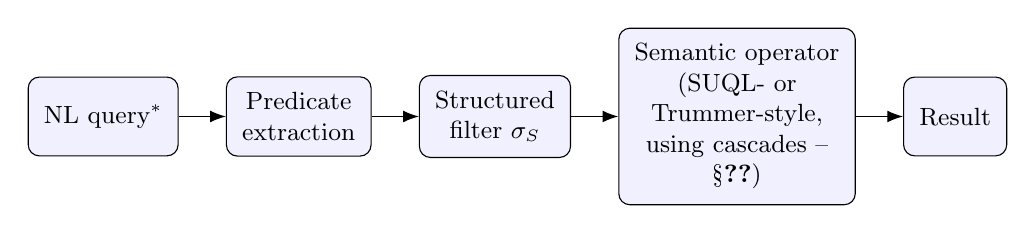
\begin{tikzpicture}[
  node distance=6mm and 6mm,
  box/.style={draw, rounded corners, align=center, minimum height=10mm, font=\small, fill=blue!6, inner sep=2mm},
  arr/.style={-{Latex[length=2mm]}}
]
\node[box] (q) {NL query$^*$};
\node[box, right=of q] (extract) {Predicate\\extraction};
\node[box, right=of extract] (sql) {Structured\\filter $\sigma_S$};
\node[box, right=of sql] (op) {Semantic operator\\(SUQL- or\\Trummer-style,\\using cascades --\\\S\ref{sec:contributions})};
\node[box, right=of op] (out) {Result};
\draw[arr] (q) -- (extract);
\draw[arr] (extract) -- (sql);
\draw[arr] (sql) -- (op);
\draw[arr] (op) -- (out);
\end{tikzpicture}
}

\vspace{2pt}
{\scriptsize $^*$Assumes $Q$ can be parsed into a structured predicate $\sigma_S$ and a semantic predicate $\sigma_U$.}
\caption{General schema of our approach.}
\label{fig:overview}
\end{figure}

\section{Cascaded Architectures}
\label{sec:contributions}
We propose two cascaded methods, \textsc{CasSuql} (\S\ref{sec:suql-v1}) and \textsc{CasTrummer} (\S\ref{sec:trummer-v1}) that are on top of \textsc{Suql} and \textsc{Trummer} respectively, together with a shared cascade calibration procedure (\S\ref{sec:cascade-math}).

Both methods rely on a cheap stage, a routing decision and an expensive stage as follows: %add the same mechanism before the semantic operator.
A cheap stage first scores every unit, where a unit is a single row for \textsc{CasSuql} and a batch of rows for \textsc{CasTrummer}. The rows for which the cheap stage is confident are considered resolved and returned immediately, and only the rows that fall inside a calibrated ambiguity band are escalated to an expensive stage. Each LLM call processes one batch, but the routing decision is made separately for every row. The cascade thus consists of two stages and a routing rule between them:
\begin{itemize}
  \item \textbf{Cheap stage.} In a single LLM call, $\mathrm{Cheap}$ estimates the probability $p = \Pr[\sigma_U(r) = \text{true}]$ for each row $r$. The probability is taken from the log-probability of the answer token (\textsc{CasTrummer}'s cheap call instead returns a \texttt{YES}, \texttt{NO} or \texttt{UNCERTAIN} label per row, which is mapped directly to $\ell = +2, -2, 0$).
  \item \textbf{Routing.} The probability is mapped to its log-odds $\ell = \log \frac{p}{1-p}$ and compared with a calibrated band $(\tau_-, \tau_+)$ (described in \S\ref{sec:cascade-math}). If $\ell \ge \tau_+$, the row is accepted, and if $\ell \le \tau_-$, it is rejected. A side of the band that calibration cannot certify is left open ($\tau_+{=}{+}\infty$ or $\tau_-{=}{-}\infty$), so that those rows are escalated rather than decided by an unverified cheap stage.
  \item \textbf{Expensive stage.} $\mathrm{Expensive}$ evaluates $\sigma_U$ with a full-context call to a larger LLM, and is invoked only for the rows with $\tau_- < \ell < \tau_+$.
\end{itemize}

% \begin{figure}[t]
% \centering
% \resizebox{\columnwidth}{!}{%
% \begin{tikzpicture}[
%   node distance=6mm and 6mm,
%   box/.style={draw, rounded corners, align=center, minimum height=9mm, font=\small, fill=blue!6},
%   dec/.style={draw, diamond, align=center, font=\small, fill=blue!6, inner sep=2pt},
%   arr/.style={-{Latex[length=2mm]}}
% ]
% \node[box] (in) {Units $u_1,\dots,u_n$};
% \node[box, right=of in] (cheap) {Stage 1: cheap $\to \ell$};
% \node[dec, right=8mm of cheap] (dec) {$\ell\in[\tau_-,\tau_+]$?};
% \node[box, above right=6mm and 8mm of dec] (exp) {Stage 2: expensive};
% \node[box, below right=6mm and 8mm of dec] (accept) {Accept/reject};
% \node[box, right=24mm of dec] (out) {Merged result};
% \draw[arr] (in) -- (cheap);
% \draw[arr] (cheap) -- (dec);
% \draw[arr] (dec) -- node[above,font=\tiny]{yes} (exp);
% \draw[arr] (dec) -- node[below,font=\tiny]{no} (accept);
% \draw[arr] (exp) -| (out);
% \draw[arr] (accept) -| (out);
% \end{tikzpicture}
% }
% \caption{Two-level cascade shared by \textsc{CasSuql} ($B{=}1$) and \textsc{CasTrummer} ($B{=}8$, batched).}
% \label{fig:cascade}
% \end{figure}

\subsection{\textsc{CasSuql}: Cascaded \textsc{Suql}}
\label{sec:suql-v1}
The algorithm is described in Alg.~\ref{alg:suql-v1}. As described above, after the structured filter, the cheap stage scores every remaining row with a single-token log-probability. Rows whose score falls outside the band are resolved without any further call, and only the rows inside the band reach a full \texttt{answer()} call, as in \textsc{Suql}. The expensive calls of \textsc{CasSuql} are therefore a subset of the ones returned by \textsc{Suql}, and \textsc{CasSuql} never issues more expensive calls than \textsc{Suql}: the calibration rows keep their expensive answer, so no row is judged twice. Its wall-clock time can still be higher, however, since the latency of the cheap stage is an overhead (\S\ref{sec:cost}).

\begin{algorithm}[h]
\caption{\textsc{CasSuql} (row-level cascade, $B{=}1$)}
\label{alg:suql-v1}
\begin{algorithmic}[1]
\Require rows $R_\sigma$ surviving $\sigma_S$; band $[\tau_-,\tau_+]$
\State $\mathrm{Ans} \gets \emptyset$
\For{$r \in R_\sigma$}
  \State $p \gets \mathrm{Cheap}(r, \sigma_U)$ \Comment{single constrained-decoding call; read \texttt{Yes}/\texttt{No} token logprob}
  \State $\ell \gets \log\frac{p}{1-p}$
  \If{$\ell \ge \tau_+$}
    \State $\mathrm{Ans} \gets \mathrm{Ans} \cup \{r\}$ \Comment{accepted on cheap score alone}
  \ElsIf{$\ell \le \tau_-$}
    \State \textbf{reject} $r$ \Comment{no further call}
  \Else
    \State $y \gets \mathrm{Expensive}(r, \sigma_U)$ \Comment{full expensive call, as \textsc{Suql}'s \texttt{answer()}}
    \If{$y = \texttt{YES}$} $\mathrm{Ans} \gets \mathrm{Ans} \cup \{r\}$ \EndIf
  \EndIf
\EndFor
\State \Return $\mathrm{Ans}$
\end{algorithmic}
\end{algorithm}

\subsection{\textsc{CasTrummer}: Cascaded \textsc{Trummer}}
\label{sec:trummer-v1}
\textsc{CasTrummer}, described in Alg.~\ref{alg:trummer-v1}, introduces three changes in the \textsc{Trummer} baseline:

\begin{enumerate}
  \item \textbf{Structured filter.} Unlike \textsc{Trummer}, $\sigma_S$ is executed in the DBMS before any LLM call (similarly to \textsc{Suql}).
  \item \textbf{Batched cheap pass with a three-way label.} Rows that pass $\sigma_S$ are grouped in batches of size $B$. As a result, every row that the LLM sees already satisfies $\sigma_S$, so no context budget is spent on rows that the DBMS can first reject at almost no cost. Following that, a single cheap call per batch returns a \texttt{YES}, \texttt{NO} or \texttt{UNCERTAIN} label for each row of the batch. Since the model is allowed to declare a row ambiguous, rows having indirect evidence are escalated instead of being labeled \texttt{NO} by default.
  \item \textbf{Batched expensive verification.} The rows whose log-odds fall inside the calibrated band, as for \textsc{CasSuql} (typically the rows labeled \texttt{UNCERTAIN}, whose score is $\ell=0$), are grouped into new batches and passed to the expensive stage. If the answer for a batch is unusable (a long prompt can overflow the context, and the model then omits row ids), the batch is split in two and each half is retried, so that no candidate is silently dropped; every retry counts as an expensive call.
\end{enumerate}

These changes allow \textsc{CasTrummer} to improve both cost and quality over \textsc{Trummer}, whereas \textsc{CasSuql} keeps the quality of \textsc{Suql} but pays a time overhead. The structured filter reduces the number of rows before any LLM call is issued. Batching  amortizes a shared prompt prefix over all rows of the same call in both the cheap and the expensive pass so that the cheap stage costs only a fraction of a full-context call to the larger LLM. Finally, the verification pass recovers the quality lost by the baseline, without processing again the rows on which the cheap pass was already confident.

\begin{algorithm}[h]
\caption{\textsc{CasTrummer} (batch-level cascade)}
\label{alg:trummer-v1}
\begin{algorithmic}[1]
\Require rows $R_\sigma$ surviving $\sigma_S$; cheap batch size $B$; expensive batch size $B'$; band $[\tau_-,\tau_+]$
\State $\mathrm{Ans} \gets \emptyset$; $\mathrm{Uncertain} \gets \emptyset$
\For{batch $b \subset R_\sigma$ of size at most $B$} \Comment{one call per batch}
  \State $\{(r, \ell_r)\}_{r \in b} \gets \mathrm{Cheap}(b, \sigma_U)$ \Comment{joint \texttt{YES}/\texttt{NO}/\texttt{UNCERTAIN} label per row, mapped to $\ell_r \in \{+2,-2,0\}$}
  \For{$r \in b$}
    \If{$\ell_r \ge \tau_+$}
      \State $\mathrm{Ans} \gets \mathrm{Ans} \cup \{r\}$
    \ElsIf{$\ell_r > \tau_-$}
      \State $\mathrm{Uncertain} \gets \mathrm{Uncertain} \cup \{r\}$ \Comment{rows with $\ell_r \le \tau_-$ are rejected}
    \EndIf
  \EndFor
\EndFor
\For{batch $b' \subset \mathrm{Uncertain}$ of size at most $B'$} \Comment{expensive re-verification}
  \State $\{(r, y_r)\}_{r \in b'} \gets \mathrm{Expensive}(b', \sigma_U)$
  \For{$r \in b'$} \If{$y_r = \texttt{YES}$} $\mathrm{Ans} \gets \mathrm{Ans} \cup \{r\}$ \EndIf \EndFor
\EndFor
\State \Return $\mathrm{Ans}$
\end{algorithmic}
\end{algorithm}

Executing $\sigma_S$ before any LLM call follows the classical query rewriting rule for expensive selections by ordering the operations ascending by $c_i/(1-s_i)$, where $c_i$ is a per-row cost and a selectivity $s_i$ is the selectivity~\cite{hellerstein1993predicate}. In our case, $\sigma_S$ is inexpensive and typically highly selective, so running it first is reasonable.

\begin{example}[Running example, continued]
Consider again the four movies of Example~\ref{ex:running} under \textsc{CasTrummer}. The structured filter $\sigma_S$ ($\text{year}=1998$) is executed in the DBMS and removes \texttt{tt0102} and \texttt{tt0103} before any LLM call. In particular, \texttt{tt0102}, the false positive of \textsc{Trummer}, can no longer be admitted, since the year check is no longer left to the LLM. The two remaining movies, \texttt{tt0100} and \texttt{tt0101}, are sent together in a single cheap call. The positive review of \texttt{tt0101} (\textit{``...crowd-pleaser...''}) is labeled \texttt{NO} and rejected (assuming the calibrated band certifies \texttt{NO} labels; otherwise it is escalated as well). The sarcastic review of \texttt{tt0100} (\textit{``...masterpiece of pure boredom...''}) contains surface praise that can mislead the cheap model; instead of guessing, the model can label it \texttt{UNCERTAIN}, in which case it is escalated to the expensive stage, which returns \texttt{YES}. The answer is $\mathrm{Ans}(Q)=\{\mathtt{tt0100}\}$, obtained with one cheap call and one expensive call.
\end{example}

\subsection{Cost Analysis}
\label{sec:cost}
We count the LLM calls issued per question, since they dominate the cost. The structured filter and the join on $\mathit{id}$, when executed by a DBMS, have a negligible cost in comparison. Let $N = |S|$ and assume one text per item ($|U| = N$). Let $s \in (0,1]$ be the selectivity of $\sigma_S$, so that $|R_\sigma| = sN$.

\textsc{Trummer} is a block nested-loop join~\cite{garcia2008database,ramakrishnan2003database} in which each pair of blocks is evaluated by a single LLM call. With blocks of $b_S$ rows of $S$ and $b_U$ texts of $U$, it issues $O(N^2/(b_S b_U))$ calls. This cost is quadratic in $N$ and does not depend on $s$ (no structured filter is applied in \textsc{Trummer}). The other three methods let the DBMS execute both $\sigma_S$ and the join, so that every row is sent to the LLM along with its candidate text. Hence, their cost is linear in the number of candidates $sN$. \textsc{Suql} issues one call per candidate, for a total of $O(sN)$ calls. \textsc{CasSuql} issues $O(sN)$ cheap calls and $O(e\,sN)$ expensive calls, where $e \in [0,1]$ is the fraction of rows escalated by the cheap stage. \textsc{CasTrummer} issues $O(sN/B)$ cheap calls and $O(e\,sN/B')$ expensive calls. Both cascades also label a calibration set with the expensive model (\S\ref{sec:cascade-math}), but those rows keep their expensive answer, so no row is judged twice. In wall-clock time, \textsc{CasSuql} pays $t_c$ per row for the cheap call and $t_e$ for the escalated rows, against $t_e$ per row for \textsc{Suql}, so it is faster exactly when $t_c/t_e < d$, where $d = 1-e$ is the fraction of rows that the cheap stage decides alone.

\subsection{Calibrating the Cascade}
\label{sec:cascade-math}

For each question, we first perform a calibration procedure using a calibration set $C$, consisting of $|C|$ rows sampled from the candidates $R_\sigma$, stratified by the confidence of their cheap stage scores, and labeled by the expensive LLM call in our implementation. The labeled rows keep their expensive answer as their final answer.

\textbf{Calibration approaches.}
Existing approaches calibrate escalation thresholds on large validation sets, using statistical accuracy guarantees~\cite{zeighami2026bargain}, isotonic regression~\cite{kotte2026ucci}, learned proxy scores~\cite{zhang2025scaledoc} or learned routing policies~\cite{chen2023frugalgpt}. In our setting, the threshold has to be recalibrated for every question from only the labeled rows in $C$. We therefore model the recall and precision of the cheap stage with Beta posteriors, which are available in closed form for any sample size and remain conservative when $|C|$ is small.

\textbf{Log-odds and the ambiguity band.} As discussed above, the cheap stage returns $p_i \in (0,1)$, which we map to its log-odds $\ell_i = \log \frac{p_i}{1-p_i}$. The band $(\tau_-,\tau_+)$ is constructed from the calibration set $C$.

\textbf{Beta-posterior bounds.}
\label{sec:beta-posterior}
For a candidate threshold $\tau$, let $\mathit{TP}(\tau)$, $\mathit{FN}(\tau)$ and $\mathit{FP}(\tau)$ be the numbers of true positives, false negatives and false positives of the cheap stage on $C$ at that threshold. With a uniform $\mathrm{Beta}(1,1)$ prior, Beta-Binomial conjugacy~\cite{gelman2013bayesian} gives the posteriors $\mathrm{Beta}(1{+}\mathit{TP}(\tau), 1{+}\mathit{FN}(\tau))$ for the recall and $\mathrm{Beta}(1{+}\mathit{TP}(\tau), 1{+}\mathit{FP}(\tau))$ for the precision of the cheap stage. We use their lower credible bounds at level $\alpha$ ($\alpha{=}0.9$ in our experiments):
\begin{align*}
  \widehat r_\alpha(\tau) &= F^{-1}_{\mathrm{Beta}(1+\mathit{TP}(\tau),\,1+\mathit{FN}(\tau))}(1-\alpha),\\
  \widehat p_\alpha(\tau) &= F^{-1}_{\mathrm{Beta}(1+\mathit{TP}(\tau),\,1+\mathit{FP}(\tau))}(1-\alpha),
\end{align*}
where $F^{-1}_{\mathrm{Beta}(a,b)}$ is the inverse CDF of $\mathrm{Beta}(a,b)$. Unlike point estimates, these bounds take into account how many calibration rows support a given threshold. Given a target quality $Q^\ast$ ($0.8$ in our experiments), the band is the narrowest one for which both bounds reach the target:
\[
  \tau_+=\min\{\tau:\widehat p_\alpha(\tau)\ge Q^\ast\}, \qquad
  \tau_-=\max\{\tau:\widehat r_\alpha(\tau)\ge Q^\ast\}.
\]
Above $\tau_+$, the precision is high enough to accept a row on its cheap score alone; below $\tau_-$, the recall is high enough to reject it; in between, the row is escalated.

\textbf{Stratified estimation.} Since $C$ is sampled across the range of cheap scores rather than uniformly, the counts above cannot be read directly from $C$. We cut the candidates into $K{=}4$ equal-count strata by cheap score (equal scores never straddle a cut), label the same number of rows in each stratum, and place an independent Beta posterior on the positive rate of each stratum. The recall and precision bounds are obtained by propagating these posteriors to the unlabeled rows of each stratum with Monte-Carlo sampling (2,000 draws), the labeled rows contributing their known answer; with a single stratum they reduce to the bounds above. The thresholds are the boundaries of the largest prefix (resp.\ suffix) of strata that clears $Q^\ast$, and a side that no stratum clears is left open, so that all rows on that side are escalated.

\textbf{Target and power.} We use $Q^\ast{=}0.8$, since $0.9$ cannot be certified from 20 labels: a cheap stage that is correct on all of them has a lower bound of only $0.896$. In simulations (300 pools per configuration, 40 to 1,000 rows, 10--30\% positives, cheap-score AUC 0.76--0.96, $|C|\in\{20,40,100\}$; script in the artifact), the true recall of a certified reject region reached $Q^\ast$ in at least 99\% of the trials, against a target of 90\%. The price is power: with $|C|{=}20$ the cheap stage decides on its own 8--13\% of the rows, and 28--36\% with $|C|{=}40$.

% \paragraph{Note.} $F^{-1}_{\mathrm{Beta}(a,b)}(y)$ is the standard inverse cumulative distribution function (quantile function) of the $\mathrm{Beta}(a,b)$ distribution: the value $x$ such that a $\mathrm{Beta}(a,b)$-distributed variable falls below $x$ with probability $y$. Equivalently, it is the inverse of the regularized incomplete Beta function $I_x(a,b)$ -- a standard special function available in any statistics package (e.g.\ R's \texttt{qbeta}).


% \textbf{Operator ordering.} For $k$ independent selection operators $O_1,\dots,O_k$, each with per-call cost $c_i$ and selectivity $s_i \in (0,1)$ (the probability a unit survives $O_i$ and still has to pass the next filter), evaluated in the order $O_{\pi(1)},\dots,O_{\pi(k)}$, the expected cost per unit is
% \[
%   \mathbb{E}[\text{cost}] = \sum_{j=1}^{k} c_{\pi(j)} \prod_{m<j} s_{\pi(m)}.
% \]
% The term $\prod_{m<j} s_{\pi(m)}$ is the probability a unit survives every operator scheduled before $O_{\pi(j)}$ and therefore actually reaches it -- an operator placed late only pays its cost on the fraction of units still standing, while one placed early pays on nearly everything. This is minimized by sorting operators by ascending $c_i/(1-s_i)$: cheap, good-rejecting filters go first, since every unit one of them rejects saves the cost of every filter waiting behind it -- the same rule ELEET~\cite{urban2024eleet} uses. That's why \textsc{CasTrummer} orders its filters structural, then cheap batch, then expensive batch: free and most-rejecting first, heaviest last.

\section{Experiments}
\label{sec:eval}

We present the experimental setup (\S\ref{sec:setup}) and the results (\S\ref{sec:results}).

\subsection{Experimental Setup}
\label{sec:setup}
\textbf{Datasets.} We use two datasets, each pairing a structured relation $S$ with a relation $U$ of user reviews.
The first is \textit{IMDb}: $S$ contains 25k movies with their title, director, release year, runtime and genres, and $U$ contains one user review per movie.
\textit{Amazon Fashion} serves as a cross-domain check, using the fashion category of the 2018 McAuley Lab release of Amazon reviews, with 186k products (title, brand, category and price) in $S$ and 882k reviews in $U$.

\textbf{Candidate pools and ground truth.} Each question is evaluated on its own pool of 100 items drawn from the corresponding corpus, with ground truth defined by $\sigma_S$ together with hand-authored regular-expression patterns that encode the semantic condition (no LLM acts as a judge). A correct paraphrase outside the patterns counts as a negative, so absolute F1 values are best read as comparisons between methods.
On \textit{IMDb}, every pool contains the four kinds of rows of Example~\ref{ex:running}: 12 answers, which satisfy both $\sigma_S$ and $\sigma_U$, 28 rows that satisfy only $\sigma_S$, 30 rows that satisfy only $\sigma_U$, and 30 rows that satisfy neither.
%Hence, 40 rows of every pool pass the structured filter, and the 30 rows that satisfy only $\sigma_U$ reveal whether a method actually enforces $\sigma_S$.
On \textit{Amazon Fashion}, every pool contains 50 products that satisfy $\sigma_S$, 15 of which are final answers.

\textbf{Questions.} Each dataset comes with a suite of ten questions (\texttt{10q}). An \textit{IMDb} question combines one or two structured conditions on the genre, the release year or the runtime with one semantic condition on the reviews.
%for instance \textit{``Which Romance movies between 90 and 130 minutes have reviews praising the characters' chemistry or relationship?''}.
The ten questions span seven genres and range from direct cues, such as \emph{funny}, to abstract and paraphrase-prone ones, such as \emph{chemistry} or \emph{approval of a twist}.
An \textit{Amazon Fashion} question restricts the type of product through its title and asks about a property described in the reviews; the ten questions are a held-out set, disjoint from the smaller suites used during development.
%for instance \textit{``Which dresses are described by reviewers as comfortable to wear?''}.

\textbf{Metrics.} We measure quality by the precision, recall and F1 of the returned set of ids with respect to the ground truth. We measure cost by the number of LLM calls, split between the cheap and the expensive model, by the wall-clock time, and by an estimated monetary cost, computed from the accelerator time at \$3 per hour. Each method is run ten times per question, and we report the mean and standard deviation over the ten questions of the per-question mean. As all calls use temperature~0, the repetitions differ only in the calibration sample.

\textbf{Models and hyperparameters.} All methods use the same two open-weight models, served with Ollama on one NVIDIA H200 at temperature~0: Gemma~4~e2b as the cheap model and Gemma~4~26b as the expensive one; the two baselines use only the expensive model.
\textsc{Suql} and \textsc{CasSuql} process one row per call ($B{=}1$). \textsc{CasTrummer} groups rows in batches of $B{=}8$ for the cheap pass and batches of $B'{=}32$ for the expensive one.
The original optimizer of \textsc{Trummer} chooses the block sizes $b_S$ and $b_U$ so that each call fits a context budget of 4,096 tokens~\cite{trummer2025semanticjoin}.
Both cascades are calibrated on $|C|{=}20$ rows per question, with $K{=}4$ strata, $\alpha{=}0.9$ and $Q^\ast{=}0.8$ (\S\ref{sec:cascade-math}). \textsc{CasSuql} reads its cheap scores from Ollama's native token log-probabilities.
Each review is also truncated before being inserted in a prompt.
For the cascades, the limits follow the length distribution of the \textit{IMDb} reviews: 1,800 characters for the cheap stage of \textsc{CasSuql}, and 3,500 for both stages of \textsc{CasTrummer}.
The expensive stage of \textsc{CasSuql} keeps the 6,000 characters of \textsc{Suql}, and \textsc{Trummer} uses 1,400.
The same limits are used for \textit{Amazon Fashion}, whose reviews are much shorter (median 270 characters, against 1,115 on \textit{IMDb})

\textbf{Artifact availability.} The source code, benchmark suites, prompts, and experiment scripts are available at \url{https://github.com/AnnaRemi/SemanticCascadedLLMJoins}.

\begin{table}[t]
\centering\footnotesize
\resizebox{\linewidth}{!}{%
\begin{tabular}{lrrrr}
\toprule
Metric & \textsc{Suql} & \textsc{CasSuql} & \textsc{Trummer} & \textsc{CasTrummer} \\
\midrule
Precision     & \underline{0.818 $\pm$ 0.213}   & \textbf{0.830 $\pm$ 0.196}   & 0.620 $\pm$ 0.313  & 0.779 $\pm$ 0.186 \\
Recall        & \underline{0.400 $\pm$ 0.207}   & \underline{0.400 $\pm$ 0.203}   & 0.275 $\pm$ 0.193  & \textbf{0.708 $\pm$ 0.189} \\
F1            & \underline{0.501 $\pm$ 0.168}   & 0.500 $\pm$ 0.153   & 0.340 $\pm$ 0.182  & \textbf{0.713 $\pm$ 0.131} \\
Wall time (s) & \textbf{24.74 $\pm$ 0.92}  & 46.98 $\pm$ 2.36 & \underline{25.39 $\pm$ 2.59}  & 25.65 $\pm$ 2.64 \\
LLM calls     & 40.00 $\pm$ 0.00   & 77.95 $\pm$ 2.84   & \underline{10.50 $\pm$ 1.27}  & \textbf{7.56 $\pm$ 0.69} \\
\bottomrule
\end{tabular}}
\caption{IMDb \texttt{10q}, Gemma: cost and quality per question, mean $\pm$ std.\ dev.\ across the 10 questions (10 reps each).}
\label{tab:results}
\end{table}

\begin{table}[tb]
\centering\footnotesize
\resizebox{\linewidth}{!}{%
\begin{tabular}{lrrrr}
\toprule
Metric & \textsc{Suql} & \textsc{CasSuql} & \textsc{Trummer} & \textsc{CasTrummer} \\
\midrule
Precision     & \underline{0.820 $\pm$ 0.115} & \textbf{0.839 $\pm$ 0.113}   & 0.565 $\pm$ 0.200   & 0.755 $\pm$ 0.285 \\
Recall        & \textbf{0.807 $\pm$ 0.254}   & \textbf{0.807 $\pm$ 0.234}   & 0.473 $\pm$ 0.260 & \underline{0.647 $\pm$ 0.325} \\
F1            & \underline{0.779 $\pm$ 0.142} & \textbf{0.796 $\pm$ 0.133}   & 0.464 $\pm$ 0.187   & 0.673 $\pm$ 0.294 \\
Wall time (s) & 29.03 $\pm$ 2.05   & 53.05 $\pm$ 2.93   & \underline{24.02 $\pm$ 5.42}  & \textbf{23.19 $\pm$ 8.37} \\
LLM calls     & 49.40 $\pm$ 0.52   & 92.00 $\pm$ 3.74   & \underline{9.00 $\pm$ 2.36}  & \textbf{8.24 $\pm$ 2.95} \\
\$-cost       & 0.0242 $\pm$ 0.0017 & 0.0442 $\pm$ 0.0024 & \underline{0.0200 $\pm$ 0.0045} & \textbf{0.0193 $\pm$ 0.0070} \\
\bottomrule
\end{tabular}}
\caption{Amazon Fashion \texttt{10q}, Gemma: cost and quality per question, mean $\pm$ std.\ dev.\ across the 10 questions (10 reps each).}
\label{tab:amazon-full}
\end{table}

\subsection{Results}
\label{sec:results}

\begin{figure}[t]
\centering
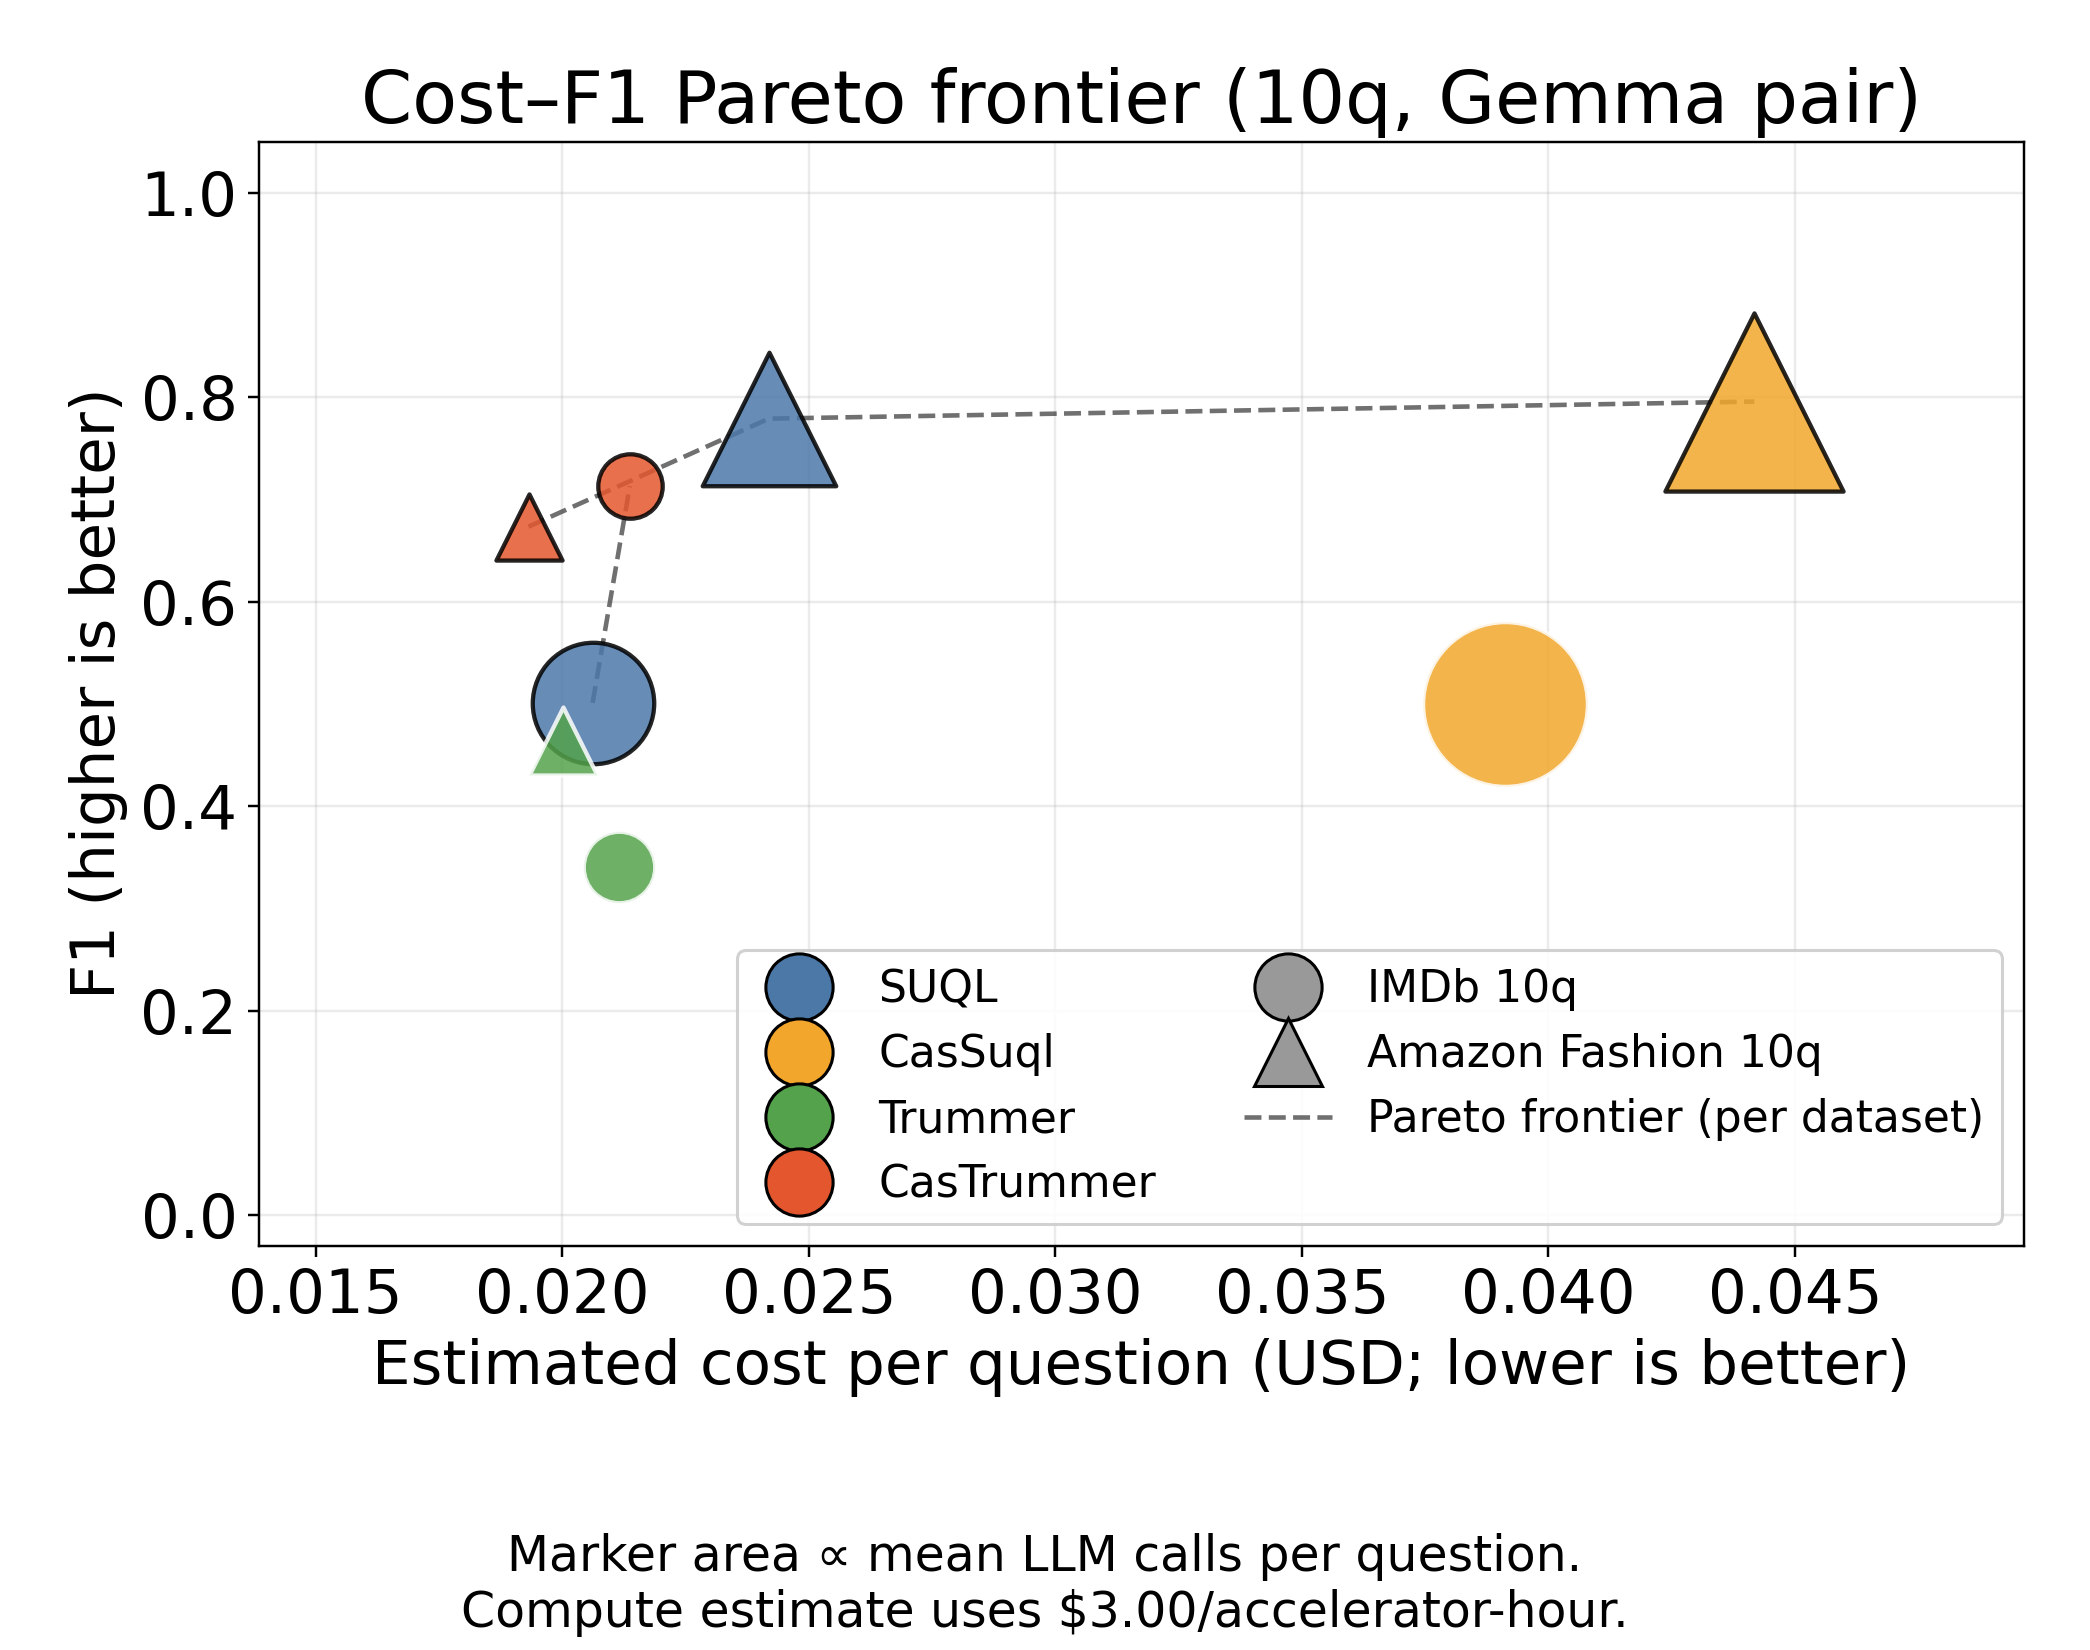
\includegraphics[width=\columnwidth]{figs/pareto/cost_f1_pareto_both_datasets.png}
\caption{Cost--F1 trade-off of the four methods on \textit{IMDb} (circles) and \textit{Amazon Fashion} (triangles), \texttt{10q} suites.}
\label{fig:pareto}
\end{figure}

\textbf{Figure~\ref{fig:pareto} (cost--quality trade-off).} Figure~\ref{fig:pareto} summarizes our results by placing the four methods in the cost--F1 plane. On \textit{IMDb}, \textsc{CasTrummer} is the most accurate method (F1 0.713 against 0.501 for the next best, \textsc{Suql}) at a dollar cost within 4\% of the cheapest one, and it uses the fewest LLM calls; \textsc{CasTrummer} and \textsc{Suql} form the Pareto front, while \textsc{Trummer} and \textsc{CasSuql} are dominated. On \textit{Amazon Fashion}, \textsc{CasTrummer} is the cheapest method, and the Pareto front also contains \textsc{Suql} and \textsc{CasSuql}, which reach a higher F1 at a higher cost. Relative to \textsc{Suql}, the strongest baseline, \textsc{CasTrummer} reduces the number of LLM calls by 81.1\% on \textit{IMDb} and 83.3\% on \textit{Amazon Fashion}, and the wall-clock time by 20.1\% on \textit{Amazon Fashion} (on \textit{IMDb} it is 3.7\% higher). The reduction in calls thus carries over from one domain to the other, whereas the quality gain does not: F1 increases by 42.3\% on \textit{IMDb} but decreases by 13.6\% on \textit{Amazon Fashion}.

\textbf{\textit{IMDb} (Table~\ref{tab:results}).} \textsc{CasTrummer} obtains the best recall and F1 with the fewest LLM calls; only its precision is below that of \textsc{CasSuql} and \textsc{Suql}. Compared with \textsc{Trummer}, it improves F1 by about 110\%, mostly through recall (from 0.275 to 0.708), and on all ten questions (paired difference $+0.373\pm0.076$), while issuing 28\% fewer calls at the same wall-clock time. \textsc{CasSuql} reproduces the quality of \textsc{Suql} (F1 0.500 against 0.501, with the same recall of 0.400 and a slightly higher precision) while sending 5\% fewer rows to the expensive model, but its wall-clock time is 1.9 times higher.

\textbf{\textit{Amazon Fashion} (Table~\ref{tab:amazon-full}).} The quality gap between the three methods that apply $\sigma_S$ is narrower: \textsc{Suql}, \textsc{CasSuql} and \textsc{CasTrummer} reach an F1 between 0.67 and 0.80, and \textsc{CasSuql} is the most accurate (0.796 against 0.779 for \textsc{Suql}, with the same recall of 0.807). \textsc{CasTrummer} remains the cheapest method in calls (83\% fewer than \textsc{Suql}), wall-clock time and dollar cost. Compared with \textsc{Trummer}, it raises F1 by 45\% (better on nine of the ten questions, paired difference $+0.209\pm0.057$), improving both precision (from 0.565 to 0.755) and recall (from 0.473 to 0.647). On one question its F1 is 0, which drives its large deviation. \textsc{CasSuql} costs 1.8 times the time of \textsc{Suql} for a gain of 0.017 F1.

\textbf{Where the gains come from.} The calibrated band is conservative. With $|C|{=}20$ labels, \textsc{CasSuql} certified a band in 34\% (\textit{IMDb}) and 77\% (\textit{Amazon Fashion}) of its repetitions, and \textsc{CasTrummer} in 18\% and 7\%; averaged over all repetitions, the cheap stage decided on its own 2.0 of 40 and 7.4 of about 50 rows for \textsc{CasSuql}, and 1.4 and 0.9 for \textsc{CasTrummer}. In every repetition in which \textsc{CasSuql} rejected rows (34 of 34 and 77 of 77), the certified recall bound was at least $Q^\ast{=}0.8$. To separate the cheap stage from the rest of \textsc{CasTrummer}, we ran it with an empty calibration set, so that every row passing $\sigma_S$ is verified by the expensive model in batches. On \textit{IMDb} this variant is as accurate (F1 0.723 against 0.713; paired difference $-0.010\pm0.035$) and 3.4\,s faster; on \textit{Amazon Fashion}, \textsc{CasTrummer} is better by $0.052\pm0.026$ at similar recall, which we cannot separate from a batch-partition effect. The quality gain of \textsc{CasTrummer} over \textsc{Trummer} (+0.38 and +0.16 for the variant) therefore comes mainly from the structured filter and the batched expensive verification, and the calibrated cheap stage adds a recall guarantee at an extra wall-clock time of 1.8--3.4\,s. For \textsc{CasSuql}, the cost model of \S\ref{sec:cost} explains the time: a cheap call took 0.58\,s against 0.62\,s for an expensive one on \textit{IMDb} (0.55 against 0.59\,s on \textit{Amazon Fashion}), so $t_c/t_e\approx0.94$, while the cheap stage decided at most $d=15\%$ of the rows, far from the break-even $t_c/t_e<d$. Each pool has only 40 or about 50 candidates, so the 20 calibration rows are 40--50\% of a pool, which limits what the cheap stage can decide alone.

\section{Conclusion and Future Work}
\label{sec:conclusion}

We proposed \textsc{CasSuql} and \textsc{CasTrummer}, which execute the structured filter in the DBMS and add a calibrated cheap stage in front of the semantic operators of \textsc{Suql} and \textsc{Trummer}. On both datasets, \textsc{CasTrummer} issues 81--83\% fewer LLM calls than \textsc{Suql} and improves the F1 of \textsc{Trummer} by 45--110\%; on \textit{IMDb} it is also the most accurate method at the wall-clock time of \textsc{Suql}, whereas on \textit{Amazon Fashion} it is the cheapest in time and dollars and trades a 14\% loss in F1 for it. An ablation shows that this quality gain comes mainly from the structured filter and the batched expensive verification. \textsc{CasSuql} preserves the quality and the recall of \textsc{Suql} with a certified bound on what its cheap stage rejects and sends fewer rows to the expensive model, but it is slower on both datasets, because the cheap model is not faster per call than the expensive one.

Future work includes a broader evaluation, with more questions, domains and model families, in particular model pairs with a larger latency gap between the cheap and the expensive model and candidate pools that are large relative to the calibration set, along with a systematic study of different batch sizes used in the joins, and possible generalization of the cascade to more than two stages.

\bibliographystyle{ACM-Reference-Format}
\bibliography{refs}
\end{document}
